% !TEX root = ../main.tex

\chapter{Literature review}
\label{ch:literature_review}

Traditionally building a computer-aider cancer diagnosis or detection (CAD) system consisted in two different parts: "Lesion  detection  and  false-positive  reduction.  Lesion  detection  was  primarily  based  on  algorithms  specific  to  the  detection task, resulting in many candidate lesions. False-positive reduction was commonly based on traditional  machine  learning  methods  to  reduce  the  false  positive  rate. However,  even  with  these  complicated and sophisticated programs, the general performance of conventional CAD systems was not good, thus hampering their widespread usage in clinical practice"\cite{41}.\\
Nowadays, this two steps tend to disappear thanks to deep learning algorithms, in particular the one based on convolutional neural networks, that constitute themselves CAD of one single step. This is the reason why CAD systems are currently a trending topic in deep learning.\\
There mainly exists two types of CAD systems based on convolutional neural networks. The first one is called CADe for "computer-aided detection". Their primary goal is "to increase the detection rate of diseases while reducing the false negative  rate  possibly  due  to  the  observers’  mistakes  or  fatigue"\cite{41}. This group includes medical  image  analysis  tasks  such  as  segmentation,  identification,  localization  and  detection. The other type is CADx for "computer-aided diagnosis" that aim to characterize the lesions.\\
This chapter goes through the main articles about CADe systems using convolutional neural networks for each body part used in the experiment of section \ref{ch:paper_reproduction} and \ref{ch:transfer_learning}, that are prostate, lung and brain. Furthermore, it focuses on articles that used the same datasets used in this work.

\section{Prostate/PROSTATEx}
"Prostate  cancer  is  the  most  common  malignancies  among  men  and  remains  a  second  leading  cause to deaths in men globally. It was predicted that there would be 1.7 million new cancer cases by 2030. The early detection and diagnosis of prostate cancer can help to survive nine out of 10 men for the last five years"\cite{41}. Therefore, researchers proposed many different models to achieve good performance in prostate cancer detection. All the articles mentioned below are based on the SPIE-AAPM-NCI PROSTATEx Challenge dataset. This dataset is composed of multiparametric MRIs (T2W, DWI, ADC, DCE, PD, Ktrans) for a total of 204 training patients which were split into a training, validation and test set (see \ref{sec:prostatex_dataset_description} for more details).\\
Song et al. \cite{07} presented a DCNN method to detect prostate cancer on multiparametric MRIs. Their data processing approach kept T2W, DWI and ADC grayscale images only. After resampling each image to the same resolution, T2W, DWI and ADC images were first cropped ($65x65$px patch) with the lesion in the center and stacked per patient, resulting in images containing three grayscale channels. Thanks to this method, the same lesion is visible in the same area over the three channels. This increases the probability of detecting a cancer by ensuring a good visibilty for each lesion, since the latter is not necesarily as visible with each parameter. Images were then normalized based on the Z-score per patient and per sequence (T2W, DWI, ADC), i.e. by subtracting the mean before dividing by the standard deviation. The training (undefined number of times), validation (undefined number of times) and test images (11x) were augmented using -20 to 20$^\circ$ rotations, horizontal flipping, vertical sliding of less than 2 pixels and stretching by a factor between 0.9 and 1.1. Most of these processing techniques were reproductible, apart from the manual lesion contouring and labelling performed by a radiologist. 
Their model is a modified version of the well-known VGG16 model, including the addition of $1x1$ convolutions and dropout layers after each max pooling layer, and the use of the ELU activation function. The evaluation method for each patient and finding made an average of the 11 predictions resulting from the 11-time augmentation of the test set. The best results were obtained by using DWI images with the highest b-value only, reaching an AUC of $0.944$ with a 95$\%$ confidence interval ($0.876$-$0.994$). However, this model was not tested on the official PROSTATEx challenge images, which is an interesting benchmark to evaluate how well a model generalizes.

Saifeng et al. \cite{31} created another architecture called XMasNet which was tested on the actual PROSTATEx challenge, achieving the second best performance at the time with an AUC of $0.84$. The AUC on their validation set reached $0.92$. Regarding data processing, their approach stacked different combinations of the available sequences as the three channels instead of defining a single combination like Song et al.: DWI-ADC-Ktrans, DWI-ADC-T2W, ADC-Ktrans-T2W and DWI-Ktrans-T2W. The data augmentation process differs in that the images are rotated in 3D, each lesion being sliced at 7 different orientations. These 2-dimensional slices were then augmented using rotation, shearing and translation of 1px, resulting in 207144 training samples. Both validation and testing test were also augmented in the same manner. This whole process allows to include 3-dimensional information in 2-dimensional images. The method used ensemble learning which combined different models the reach the best performance possible. 

Mehrtash et al. \cite{01} used a different approach. First of all, the input was feeded to three separated parts of the model, each one responsible for a specific sequence among ADC, maximum b-value DWI and Ktrans. Then, each of these feature extractors' outputs were merged into a common decision maker. Furthermore, 3-dimensional convolutions instead 2-dimensional ones were performed. In fact, 3-dimensional patches centered on the lesion were cropped. Augmentation including translation and flipping was used in order to balance the dataset. Apart from these differences, other minor differences such as normalizing the images within the range $[0,1]$ exist compared to the previous papers. These tricks allowed their model achieved an AUC of $0.80$ on the PROSTATEx challenge. To make predictions, five different models were used, averaging the predictions of the four best models. 

Armato et al \cite{42} summarized the results obtained by all teams that took part in the PROSTATEx challenge in 2017. This challenge was split into two tasks. The first one was devoted to the diagnostic classification of prostate lesions whereas the other was about the segmentation and the determination of Gleason Grade Group. Thirty-two group submitted results to the first challenge from a total of 71 different methods (each group was allowed to submit results up to three methods). The article indicates that "most, but not all, methods outperformed random guessing (AUC=0.5)"\cite{41}. The best performing method obtained an AUC value of 0.87 (standard error 0.027) and the next three methods all achieved AUC values of 0.84 (with standard errors of 0.036, 0.032, and 0.032). Globally, all results are illustrated on figure \ref{fig:challenge_all_results}. The median AUC on the challenge is approximately at 0.68.
\begin{figure}[!h]
\centering
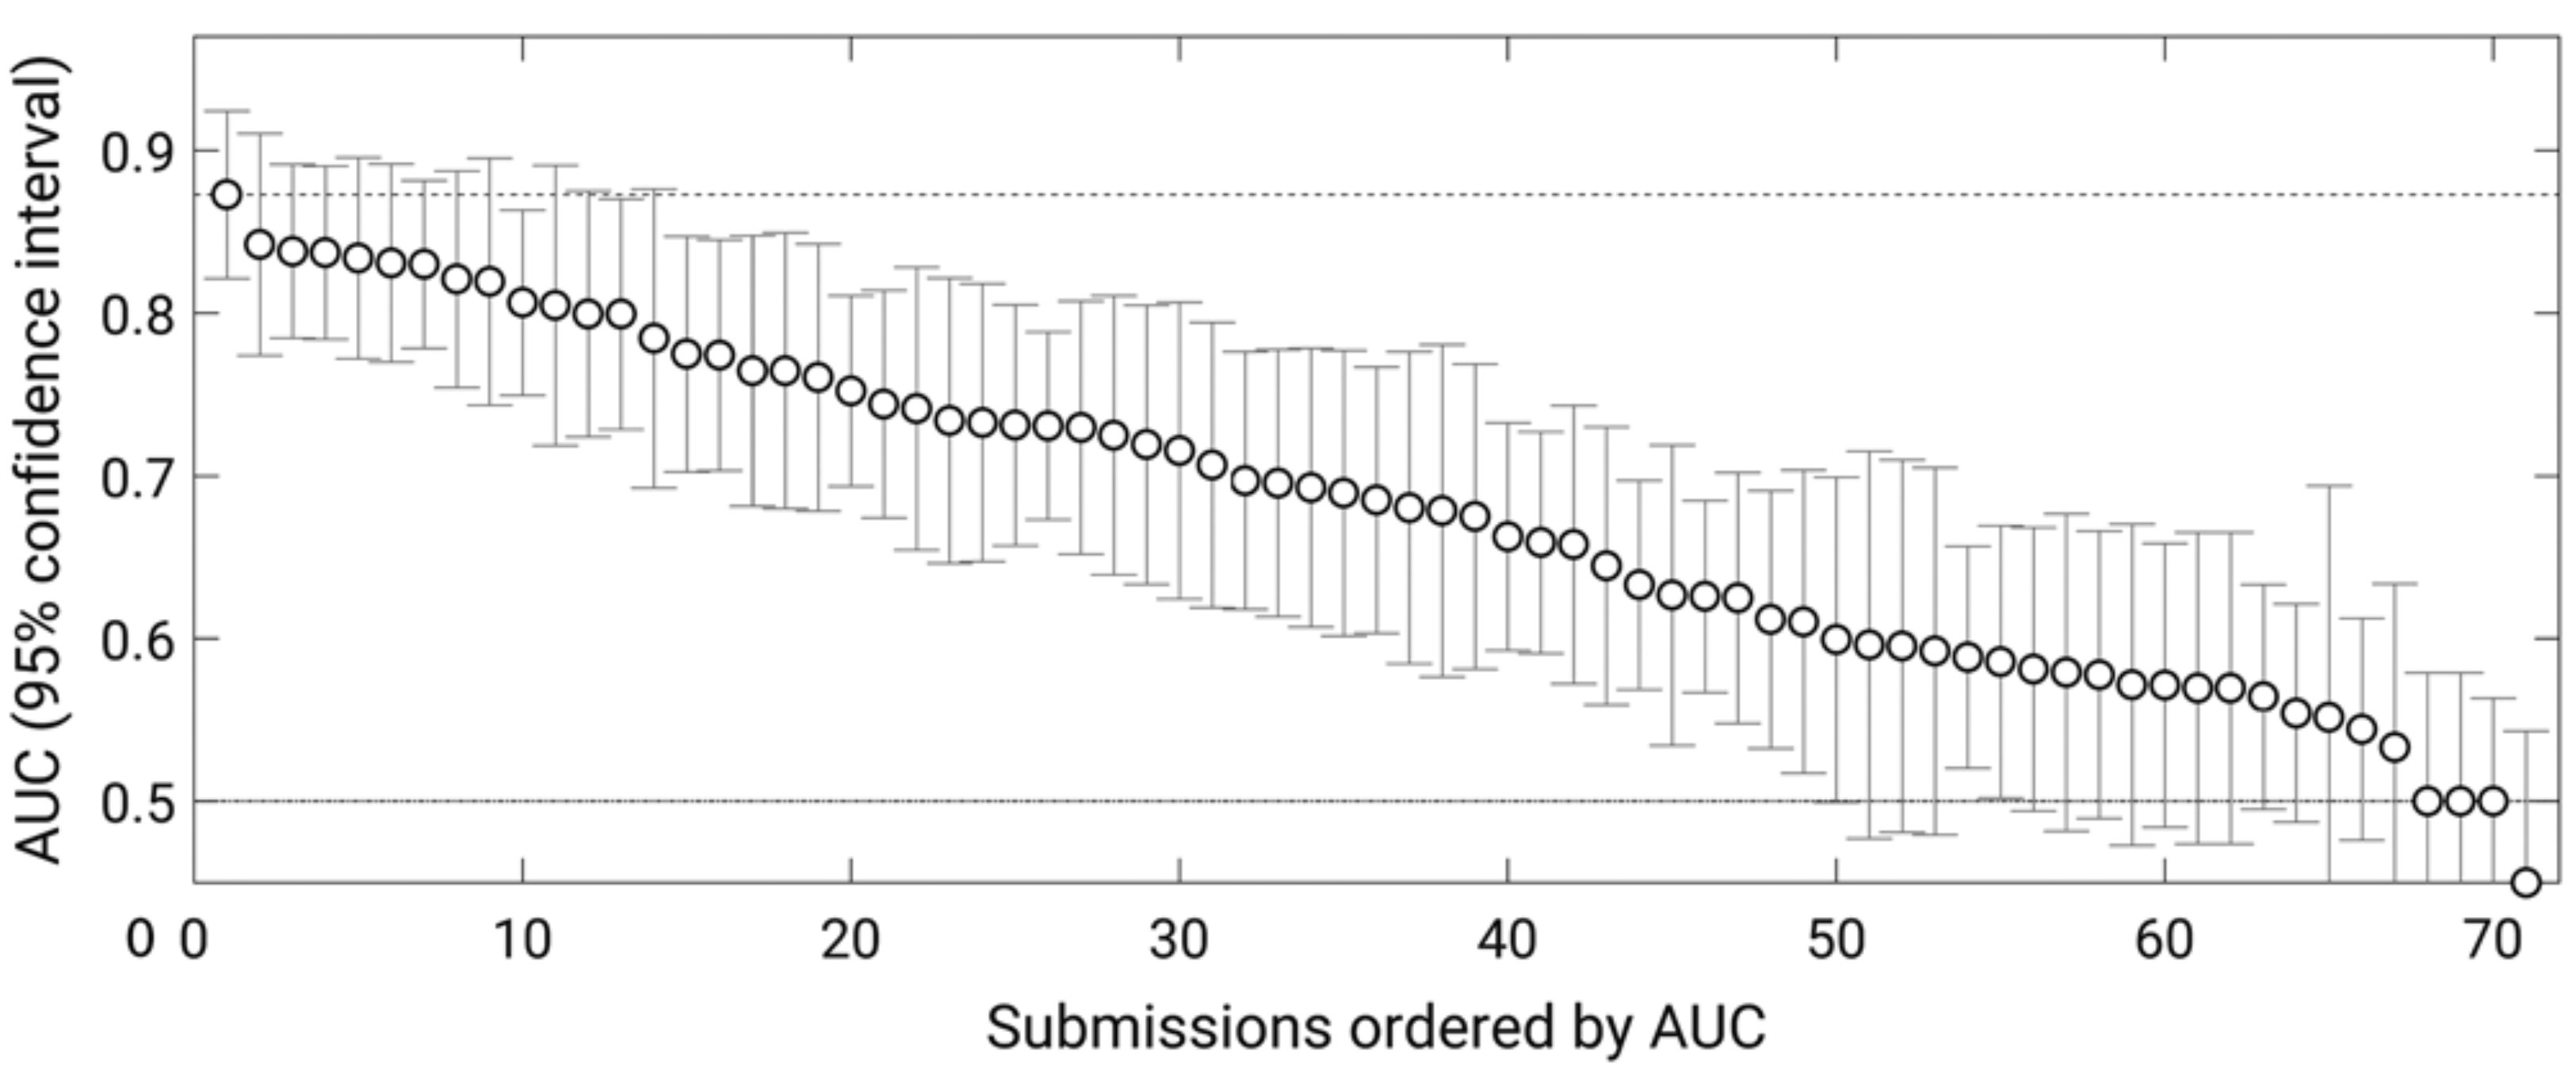
\includegraphics[width=1\textwidth, keepaspectratio=true]{./figures/challenge_all_results.png}
\caption{AUC values achieved by the 71 methods that participated in the PROSTATEx Challenge }
\label{fig:challenge_all_results}
\end{figure}


\section{Lung/Lung CT Challenge}
"Lung cancer is one of the most frequent and leading causes to death all over the world. It was reported that there were approximately $1.8x10^6$ new cases of lung cancer globally in 2012. Early detection of lung cancer, which is typically viewed in the form of lung nodules, is an efficient way to improve the survival rate"\cite{41}. All the articles cited below make use of the SPIE-AAPM Lung CT Challenge dataset, which is a dataset of CT scans devoted to the classification of lung nodules (see \ref{sec:lungCTChallenge} for more details).

Cengil et al. \cite{02} built a fairly simple convolutional neural network to classify images of the Lung CT Challenge dataset. The model takes 4-dimensional data as input (depth, height, width and channels) and performs 3D convolutions on it. The model consists of an input layer, five layers of 3D convolutions (the first is associated with a RELU activation function and pooling, the last with nothing, and the others with pooling) and a fully connected layer at the end. Regarding the model evaluation, authors announce an accuracy of 0.7 on their test set, composed of 30 findings.\\
Armato et al. \cite{12} described the LUNGx Challenge and their results. This challenge consisted in classifying the lung nodules as benign or malignant among a training set of 10 scans and a test set of 60 scans. Since the training set was extremely small, training the model on other datasets was allowed.  The article describes the results of the proposed methods and compare them with the performance of six radiologists on the same task. The article reports that: "ten groups applied their own methods to 73 lung nodules (37 benign and 36 malignant) that were selected to achieve approximate size matching between the two cohorts. Area under the receiver operating characteristic curve (AUC) values for these methods ranged from 0.50 to 0.68. Only three methods performed statistically better than random guessing. The radiologists’ AUC values ranged from 0.70 to 0.85. Three radiologists performed statistically better than the best-performing computer method."\cite{12}. Figure \ref{fig:LUNGx_challenge_all_results} gives an overview of all results.

\begin{figure}[!h]
\centering
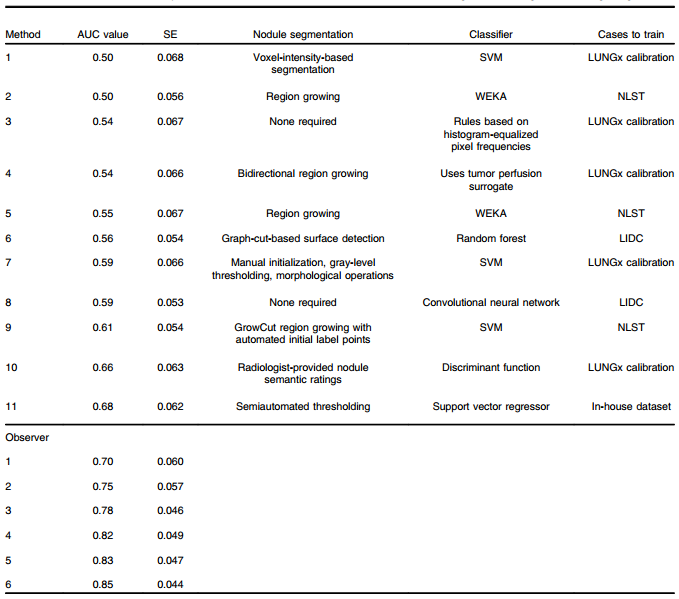
\includegraphics[width=1\textwidth, keepaspectratio=true]{./figures/LUNGx_challenge_all_results.png}
\caption{AUC values for the 11 computerized methods and six radiologists in the task of classifying malignant and benign nodules}
\label{fig:LUNGx_challenge_all_results}
\end{figure}



\section{Brain/Kaggle Brain}
Brain cancer is another major type of cancer. "Brain and other nervous system cancer is the 10th leading cause of death for men and women. It is estimated that 17760 adults (9910 men and 7850 women) will die from primary cancerous brain and central nervous system tumors this year"\cite{43}. All the following articles are based on the Kaggle Brain dataset. This dataset, unlike the ones for the prostate and the lung, does not come from a certified medical authority but from the Kaggle website. However, since it is the only dataset available for the brain tumor classification, some publications used it (see \ref{sec:kaggleBrain} for more details).

Saxena et al. \cite{31} implemented three convolution neural networks to classify the brain tumors coming from the Kaggle "Brain MRI Images for Brain Tumor Detection" dataset. Their processing method used a cropping technique which removed extra black margin around the skull. Each border of the image merges with a part of the skull. Since the images come from different sources, their resolution vary quite a lot. Therefore, the authors resized them to $224x224x3$. Moreover, data was augmented by rotation and vertical/horizontal shifting. As the cropping was performed before augmenting the images, small parts of the brain are outside of the augmented images due to rotation and shifting. The data was split into a training set, a validation set and a test set. Regarding the models, authors implemented three of them (a Resnet-50, a VGG-16 and an Inception-V3) in order to compare their performance. The best results on the test set were achieved by the Resnet-50 (AUC of $0.95$ and accuracy of $0.95$). The VGG-16 was close (AUC of $0.90$ and accuracy of $0.90$), whereas the Inception-V3 didn't perform well (AUC of $0.55$ and accuracy of $0.55$).

%Hanwat et al. \cite{32} implemented a convolutional neural network to classify brain tumors of the Kaggle dataset. Their processing method included skull masking, i.e. the removal of every non-brain tissue from the image. According to the authors, this technique improves performance quite a lot. ---> Check their methods (graphs look special)

Habib Mohamed Ali \cite{04} proposed a self created convolutional neural network to classify the images of the Kaggle Brain dataset. First, the data was augmented. Then, it was cropped to contain only the brain, resized and normalized in order to scale pixel values to the range [0,1]. After the preprocessing, the data was split into a training set (70\%), a validation set (15\%) and a test set (15\%). Regarding the neural network structure, the model is simple. It is composed of only one convolutional layer with a batch norm layer and ReLu activation function, followed by two max pool layers and a dense layer. Thanks to this model, an accuracy of 89\% was achieved on the test set.

